\documentclass{report}
\usepackage[margin=1in]{geometry}
\usepackage{setspace}
\usepackage{times}
\title{
	\textsc{ \small
		Washington State University \\
		School of Electrical Engineering and Computer Science \\
		EE 352, Electrical Engineering Laboratory
	} \\
	{\textsc{\small Lab \#6}} \\
	Transfer Function Analysis
}

\author{
	Name: Kevin Evans \\
	Partner: Jacob Hnatiak, Aman Amad al-Ameedi
}
\date{Due Date: March 3, 2020}


% start sections at 1 with subsections to 1.1, 1.2...
\renewcommand{\thesection}{\arabic{section}}

%alias for vpp/rms
\newcommand{\pp}{_{pp}}
\newcommand{\rms}{_{rms}}
\newcommand{\Vpp}{\V\pp}
\newcommand{\Vrms}{\V\rms}

\usepackage{siunitx}
\usepackage{threeparttable}
\usepackage{booktabs}
\usepackage{multirow}
\usepackage{graphicx}
\usepackage{float}
\usepackage{amssymb,amsmath}
\usepackage{physics,cancel}
\usepackage{listings}
\usepackage{steinmetz} % \phase{}
\usepackage{mathtools} % for '\mathclap' macro
\usepackage{caption,subcaption} %multiline captions; subfigures


\begin{document}
\maketitle

\section*{Lab Overview}
% what was the lab about and the outcome?
In this lab, we used transfer functions as a way to describe second-order circuits and determine the frequency and step responses. This was done for a second-order RLC high-pass filter and Butterworth low-pass filter. Later, the filters were combined to create a wide bandpass filter.

%%%%%%%%%%%%%%%%%%%%%%%%%%%%%%%%%%%%%%%%%%%%%%%%%%%%%%%%%%%%%
\section{Second-order RLC high-pass filter}
\subsection{Purpose}
% purpose of the experiment and its specs and/or design requirements
In this experiment, we determined the transfer function for a second-order RLC high-pass filter (HPF) and estimated the amplitude and phase responses, and later the step response. The circuit was built and the experimental responses were obtained.

\subsection{Theoretical background}
% background and its theory of operation, circuit diagrams, the main equations, results from the prelab
The passive high-pass filter circuit, shown in Figure \ref{fig:exp1ckt}, can be described using a transfer function. This can be done by using the impedances of each component and applying a voltage-divider technique to find the output $v_o$, \begin{align}
	V_o(s) & = \frac{Z_L}{Z_R + Z_C + Z_L} V_i(s) \notag \\
	H(s) & = \frac{sL}{R + 1/sC + sL} \notag \\
		& = \frac{s^2}{s^2 + sR/L + 1/LC}
\end{align}
If we let $s=j\omega$, we can confirm the high-pass behavior at the limiting cases, \begin{align*}
	\lim_{\omega \to 0} H(s) & = 0 && \text{(blocking DC)} \\
	\lim_{\omega \to \infty} H(s) & = 1 && \text{(pass high freq.)}
\end{align*}
If we convert the denominator to standard form, \begin{subequations}
	\begin{align}
		D(s) & = s^2 + 2 \zeta \omega_n s + \omega_n^2 \\
		2 \zeta \omega_n & = R/L 	\label{eq:exp1zeta} \\
		\omega_n^2 & = 1/LC 	\label{eq:exp1omega}
	\end{align}
\end{subequations}

\noindent This lab requires a natural frequency of $f_n = \SI{20}{\kHz}$ and a damping factor $\zeta = 0.2$. This was done by determining the component values needed to achieve these specifications, using \eqref{eq:exp1zeta} and \eqref{eq:exp1omega}. As the inductor was the limiting factor, as only two are available on-hand, the inductor value was chosen to be \SI{1}{\milli\henry}. The other component values were then calculated as,
\begin{align*}
	\omega_N = 2 \pi f_n & = \frac{1}{\sqrt{LC}}  \\
		2\pi \left( \SI{20}{\kHz}\right)& = \frac{1}{\left(\SI{1}{\milli\henry}\right) C} \\
	\Aboxed{ C & = \SI{63.3}{\nano\farad}} \\
	2 \zeta \omega_n & = \frac{R}{L} \\
		2 (0.2) \left(2 \pi f_n\right) & = \frac{R}{\SI{1}{\milli\henry}} \\
		\Aboxed{ R & = \SI{50.26}{\ohm} }
\end{align*}
\begin{figure}[h]
	\centering
	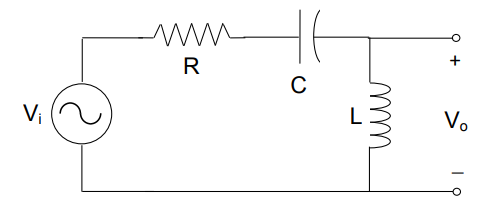
\includegraphics[width=0.4\linewidth]{exp1_ckt}
	\caption{The passive high-pass filter circuit used in Experiment 1.}
	\label{fig:exp1ckt}
\end{figure}
\noindent Using MATLAB, the system was simulated as shown in Figure \ref{fig:exp1_matlab}. A sinusodial response is shown in the Bode plot and the step response was simulated as well. The code is listed in the Appendix. Additionally, the circuit was drawn in OrCAD and simulated using PSPICE within the suite. The frequency response and step response is shown below in Figure \ref{fig:exp1_orcad}.

\begin{figure}[H]
	\centering
	\begin{subfigure}{0.45\textwidth}
		\centering
		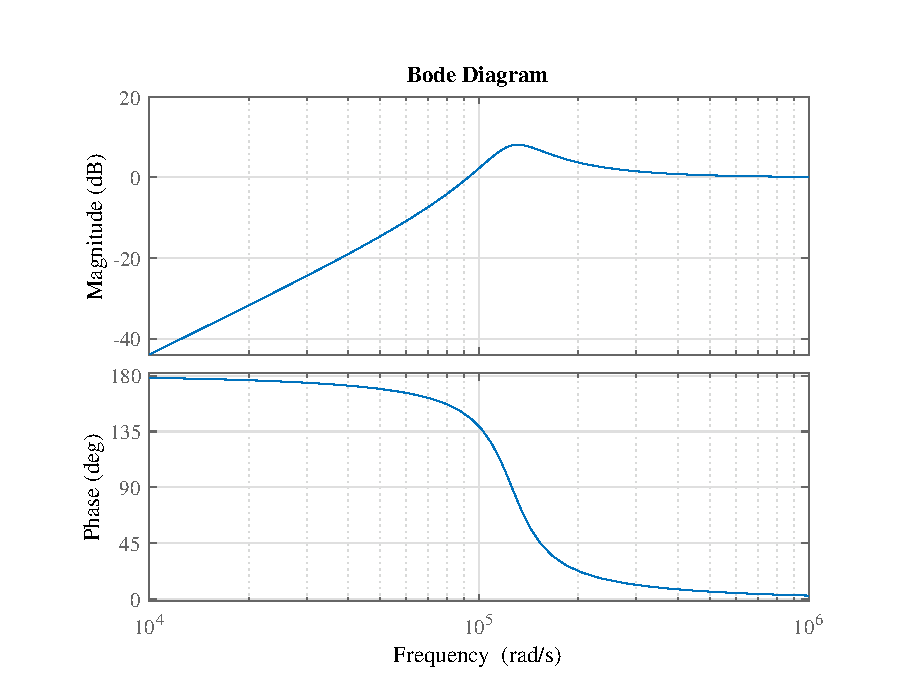
\includegraphics[width=\linewidth]{exp1_matlab_bode}
		\caption{}
	\end{subfigure}
	\begin{subfigure}{0.45\textwidth}
		\centering
		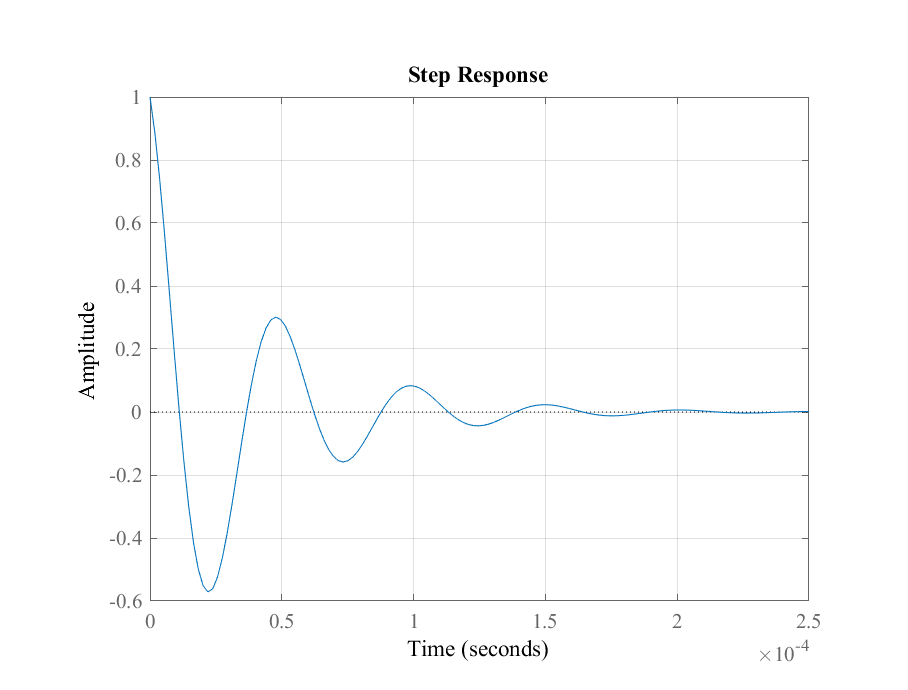
\includegraphics[width=\linewidth]{exp1_matlab_step}
		\caption{}
	\end{subfigure}
	\caption{Using the Control Systems toolbox within MATLAB, the (a) frequency response and (b) step response were captured of the circuit.}
	\label{fig:exp1_matlab}	
\end{figure}

\begin{figure}[H]
	\centering
	\begin{subfigure}{0.45\textwidth}
		\centering
		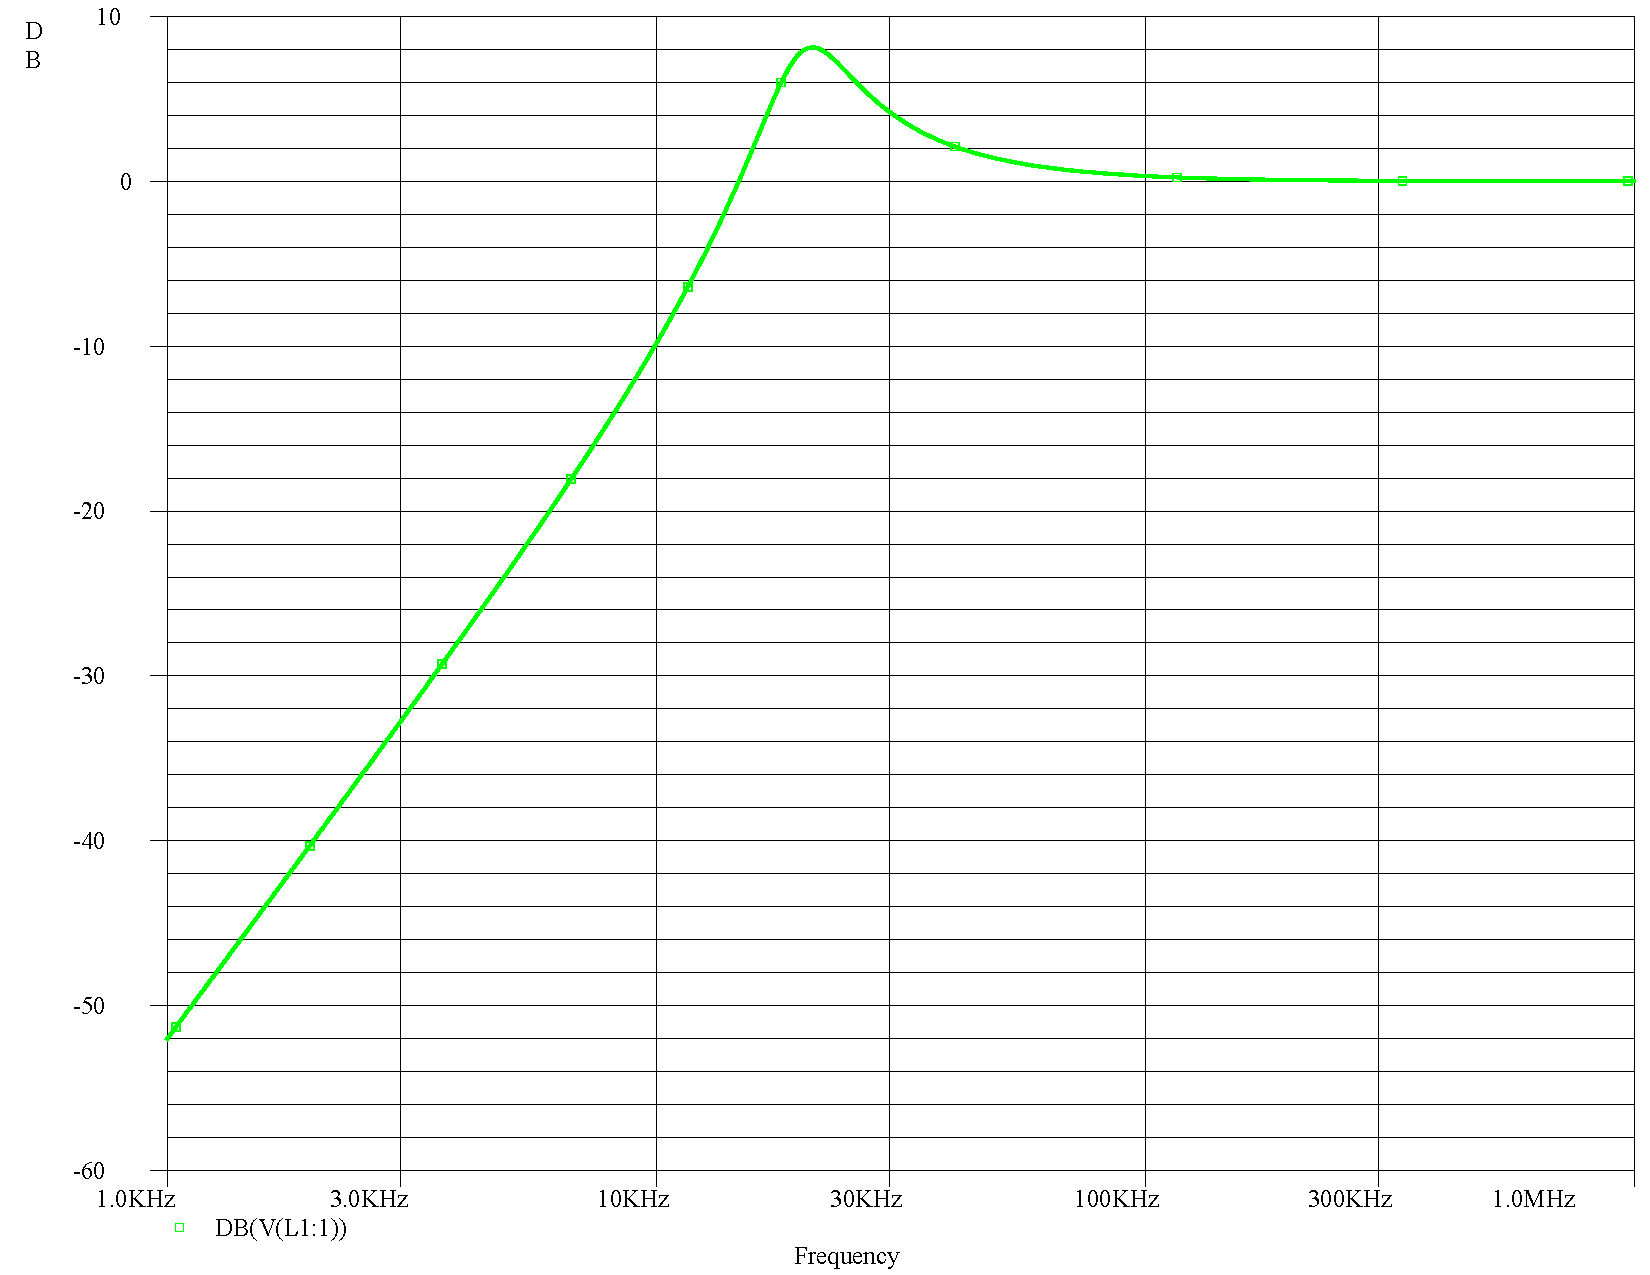
\includegraphics[width=\linewidth]{exp1_orcad_bode}
		\caption{}
	\end{subfigure}
	\begin{subfigure}{0.45\textwidth}
		\centering
		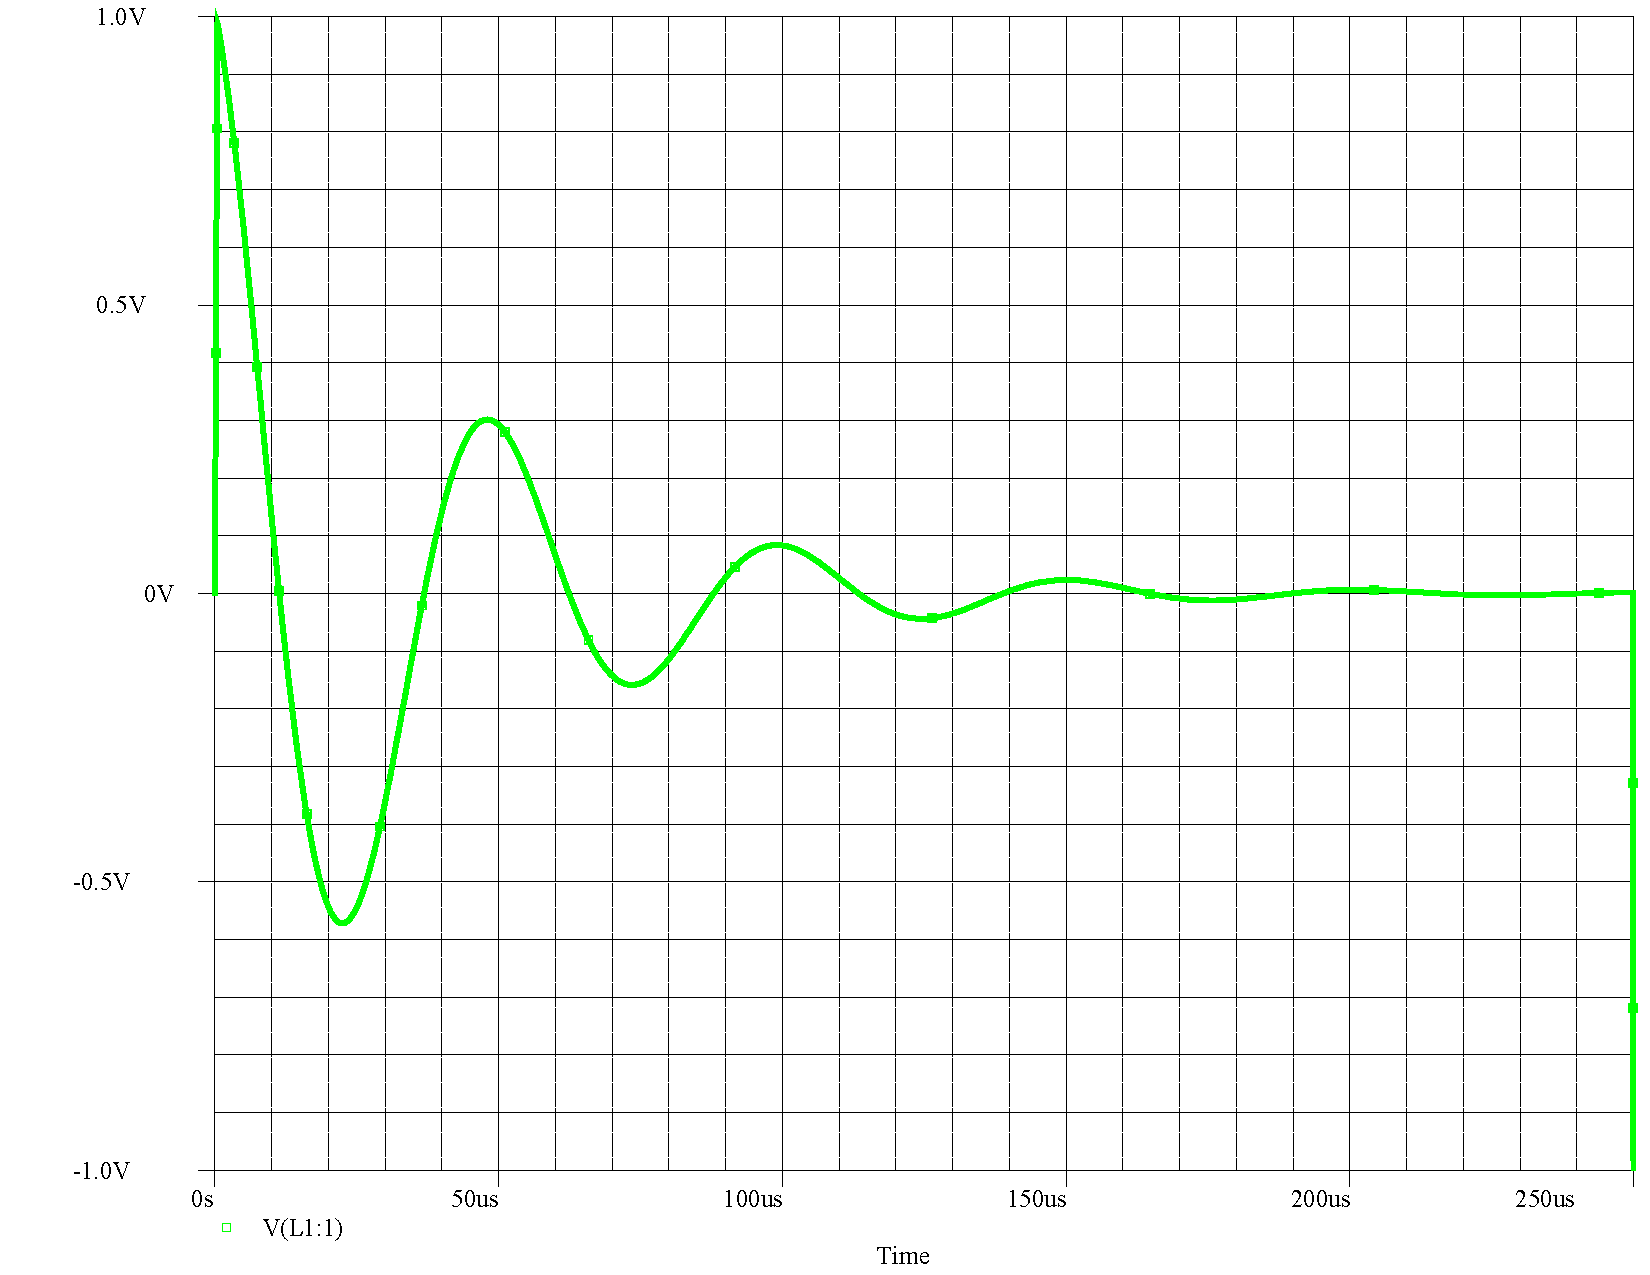
\includegraphics[width=\linewidth]{exp1_orcad_step}
		\caption{}
	\end{subfigure}
	\caption{Using PSPICE within the OrCAD Capture Lite suite, the (a) frequency response and (b) step response were captured.}
	\label{fig:exp1_orcad}	
\end{figure}

\subsection{Procedure}
The follow steps were carried out, as instructed by the lab assignment.
\begin{enumerate}
	\item The circuit shown in Figure \ref{fig:exp1ckt} was constructed using the nominal component values \begin{align*}
		R & = \SI{50.26}{\ohm} \\
		L & = \SI{1}{\milli\henry} \\
		C & = \SI{63.3}{\nano\farad}
	\end{align*}
	These components were approximated and the actual values were measured and recorded.
	
	\item The experimental frequency response was measured and recorded. This was done by using a sine wave of \SI{8}{\Vpp} as the input. The output amplitude was measured using the oscilloscope as well as the change in phase (in time). The time difference in the input and output sine wave $\Delta T$ was converted to degrees. This data was recorded in Excel and plotted using a log scale. 
	
	\item The experimental step response was measured and recorded. We achieved this by using a \SI{1}{\Vpp} sine wave with a \SI{0.5}{\V} offset, i.e. simulating \SI{0}{\V} until a time where the input voltage jumps to \SI{1}{\V} with a nearly instantaneous rise-time. The \SI{50}{\ohm} resistor was left out, as the internal resistance of the function generator was \SI{50}{\ohm}.
	
	\item The circuit was demonstrated to the TA.
	\item The RLC circuit was left on the board and the next experiment was constructed on an unpopulated breadboard.
\end{enumerate}

\subsection{Results and analysis}
% state all measured values, graphs, tables, and figs.
% state any deviation from theoretical expected values
% use tables and graphs
% * must justify error in results otherwise the experiment failed

\subsubsection{Measured component values}
The components used in this experiment were measured and are shown in Table \ref{table:exp1components}. The resistor was measured using the DMM. The inductor and capacitor were measured using the RLC meter.
\begin{table}[h]
	\centering
	\caption{Experimental and nominal component values.}
	\label{table:exp1components}
	\begin{threeparttable}
		\begin{tabular}{cccc}
			\toprule
			Component & Nominal & Experimental & \% Error (Tolerance) \\
			\midrule
			$L$  & \SI{1}{\milli\henry} & \SI{1.0458}{\milli\henry} & 4.6\%  \\
			$R$ & \SI{50.3}{\ohm} & \SI{50.88}{\ohm} & 1.2\% (5\%) \\
			$C$\tnote{*} & \SI{63.3}{\nano\farad} & \SI{61.4}{\nano\farad} & 3.0\% \\
			\bottomrule
		\end{tabular}
		\begin{tablenotes}
			\item[*] As a \SI{63.3}{\nano\farad} capacitor was unavailable, the equivalent capacitance was made by a parallel combination of: \SI{41}{\nano\farad}, \SI{11}{\nano\farad}, \SI{4.8}{\nano\farad}, \SI{4.7}{\nano\farad} capacitors.
		\end{tablenotes}
	\end{threeparttable}
\end{table}

\subsubsection{Frequency response}
The function generator was set to output a sine wave. During this experiment, both the input and output peak-to-peak voltages were recorded, as well as the difference in peak-to-peak times. The experimental bode plot is shown below in Figure \ref{fig:exp1bode}. Although the angle of the low-frequency response would be ideally flat near $180^\circ$, it likely dropped due to the low time resolution and difficultly finding the peaks of the low-amplitude sine waves.

\begin{figure}[h]
	\centering
	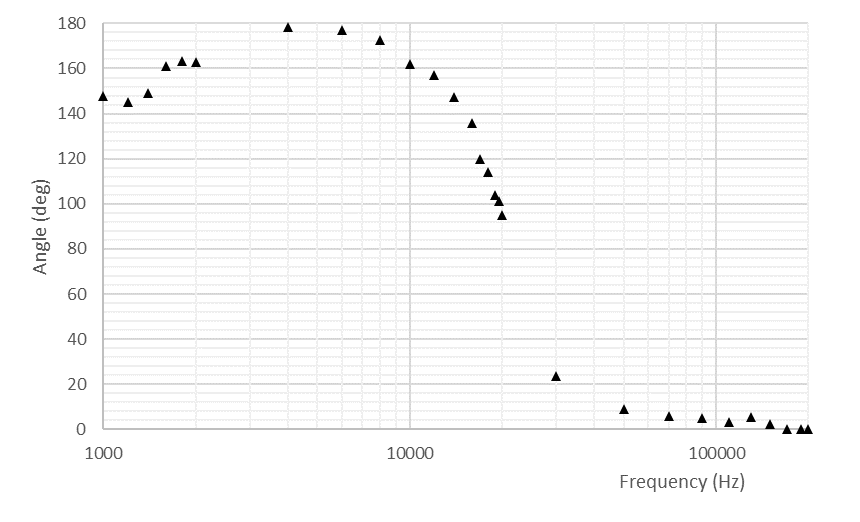
\includegraphics[width=0.5\linewidth]{exp1_freq_angle}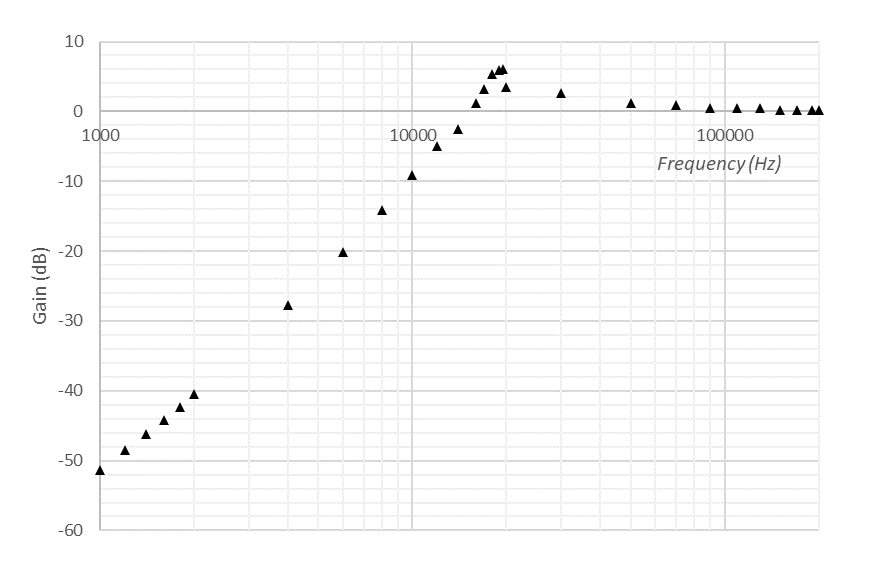
\includegraphics[width=0.5\linewidth]{exp1_freq_angle1}
	\caption{Experimental Bode plot of the frequency response of the RLC circuit.}
	\label{fig:exp1bode}
\end{figure}

The non-ideal simulations of PSPICE show a maximum gain \SI{8.13}{\dB} at \SI{20.9}{\kHz} and falls to unity gain as the frequency increases afterwards. The MATLAB simulation shows a similar picture. Relative to the simulated responses of \ref{fig:exp1_matlab} and \ref{fig:exp1_orcad}, the actual peak gain is slightly lessened. The experimental filter peaks around \SI{19500}{\dB} at a lowered gain of \SI{6.1}{\dB}. From the natural frequency in the specifications, \SI{20}{\kHz}, this is 2.5\% error. The difference is likely due to the non-ideal nature of the system and the small errors in the component values.

\subsubsection{Step response}
The step response was done using a square wave input on the function generator. In this experiment, the \SI{50}{\ohm} resistor was removed as the function generator has \SI{50}{\ohm} impedance internally. Using cursors shown in Figure \ref{fig:f0003tek}(b), the valley-valley time and frequency was measured as \begin{align*}
	\Delta T & = \SI{47.06}{\us} \\
	f & = 1 / \Delta T = \SI{21.2}{\kHz}
\end{align*}
Relative to the simulations, which achieve a natural frequency of \SI{20}{\kHz}, the measured frequency from the step response has a relative high error of 6.0\%. Again, this can be attributed to the error in component values. Additionally, the lower trough of the second wave was likely at a time past our marked time. There was difficulty determining the true minimum of the trough, mostly due to the high noise in the signal and decreasing amplitude.
\begin{figure}[h]
	\centering
	\begin{subfigure}{0.4\textwidth}
		\centering
	\includegraphics[width=\linewidth]{"Lab 6 Pics/F0002TEK"}
		\caption{}
	\end{subfigure}
	\begin{subfigure}{0.4\textwidth}
		\centering
		\includegraphics[width=\linewidth]{"Lab 6 Pics/F0003TEK"}
		\caption{}
	\end{subfigure}
	\caption{Screenshots of the step response. (a) The step response until equilibrium and (b) the cursors demonstrating the valley-valley time measurement.}
	\label{fig:f0003tek}
\end{figure}
\subsection{Conclusion}
%  conclusion of the exp
This experiment experimentally confirmed the high-pass response of a series RLC circuit and showed two methods of determining the natural response. Additionally, the experiment showed two methods of simulating the responses: one using OrCAD PSPICE and the other with MATLAB. The experiment used transfer functions to model the circuit as an equation in the $s$-domain, allowing us to easily determine the rough behavior of the circuit and fit it to existing models.

%%%%%%%%%%%%%%%%%%%%%%%%%%%%%%%%%%%%%%%%%%%%%%%%%%%%%%%%%%%%%
\section{Second-order active Butterworth low-pass filter}

\subsection{Purpose}
% purpose of the experiment and its specs and/or design requirements
The purpose of this experiment was to design and build a second-order active Butterworth low-pass filter. This filter will have a characteristic smooth Butterworth curve, allowing a smooth transition between the low-pass and high-frequency blocking regions.

\subsection{Theoretical background}
% background and its theory of operation, circuit diagrams, the main equations, results from the prelab
This experiment focuses on using a second-order Butterworth filter. These filters are described the transfer function, which have a magnitude of the form of \begin{align}
	\abs{H(jw)} & = \frac{1}{\sqrt{1 + \left(\omega / \omega_c\right)^{2N}}} \label{eq:exp2magnitude}
\end{align}
The $N$ poles of this transfer function are given as \begin{align}
	s_k & = \omega_c e^{j \pi / 2} e^{j\left(2k + 1\right)\pi / 2N} & k = 0, 1, N - 1 \label{eq:exp2poles}
\end{align}
For a cutoff frequency $\omega_c$, stopband frequency $\omega_s$ with attenuation $\delta_2$, the filter's order is determined as \begin{align}
	N & = \left\lceil \frac{\ln[(1 / \delta_2)^2 - 1]}{2\ln(\omega_s / \omega_c)} \right\rceil \label{eq:exp2n}
\end{align}
The Butterworth filter circuit is shown in Figure \ref{fig:exp2ckt} below. The filter's parameters are specified by selecting the component values and equating the transfer function below.
\begin{figure}[H]
	\centering
	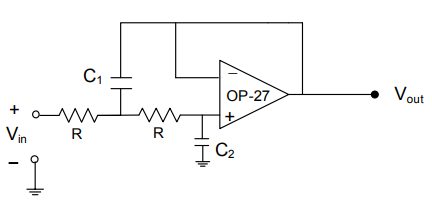
\includegraphics[width=0.4\linewidth]{exp2_ckt}
	\caption{The Butterworth low-pass filter used in Experiment 2.}
	\label{fig:exp2ckt}
\end{figure}
\noindent It can be shown that this circuit with natural frequency $\omega_n$ and damping factor $\zeta$ has a transfer function of the form \begin{align}
	H(s) & = \frac{1 / \left( R^2 C_1 C_2\right)}{s^2 + s \left(2/RC_1\right) + 1 / \left(R^2 C_1 C_2\right)} = \frac{\omega_n^2}{s^2 + 2 \zeta \omega_n s + \omega_n^2} \label{eq:exp2h}
\end{align}
The specifications of this experiment require a cutoff frequency $f_c = \SI{80}{\kHz}$, stopband frequency $f_s = \SI{300}{\kHz}$ with attenuation \SI{-20}{\dB}. For these requirements, we first determine the order using \eqref{eq:exp2n}, \begin{align*}
	N & = \left\lceil \frac{\ln(1/0.01 - 1)}{2 \ln(300/80)} \right\rceil = 2
\end{align*}
From this, we can find the two poles with \eqref{eq:exp2poles}, \begin{align*}
	s_k & = \omega_c \left( -\frac{1}{\sqrt{2}} \pm \frac{1}{\sqrt{2}}\right) \\
		& \approx -335.43 \pm j335.45 \; \si{\kilo \radian\per\s}
\end{align*}
Next, we can determine the component values using the denominator of \eqref{eq:exp2h} and equating the components to the requirements of the filter. Here, we take the capacitor $C_1$ to use \SI{10}{\nano\farad} per the in-class discussion, \begin{align*}
	\sqrt{2} \omega_c & = 2 \zeta \omega_n = \frac{2}{RC_1} \\
	\sqrt{2} \left(2 \pi \times \SI{80}{\kHz}\right) & = \frac{2}{R \left(\SI{10}{\nano\farad}\right)} \\
	\Aboxed{ R & =  \SI{281.35}{\ohm}}
\end{align*}
Using the given natural frequency and equating the polynomials again, \begin{align*}
	\omega_n^2 & = \omega_c^2 = \frac{1}{R^2 C_1 C_2} \\
	\left(2 \pi \SI{80}{\kHz}\right)^2 & = \frac{1}{\left(\SI{281.35}{\ohm}\right)^2 \left(\SI{10}{\nano\farad}\right) C_2} \\
	\Aboxed{C_2 & = \SI{5}{\nano\farad}}
\end{align*}
Again, we can use MATLAB to simulate the approximate response of the circuit. This was done using the code provided in the Appendix. The response is shown below in Figure \ref{fig:exp2_matlab}. Additionally, the responses were simulated in OrCAD PSPICE and displayed in Figure \ref{fig:exp2_orcad} below. Both simulations show the expected Butterworth curves, with the magnitude of the frequency response smoothly transitioning between the bandpass region. 
\begin{figure}[H]
	\centering
	\begin{subfigure}{0.4\textwidth}
		\centering
		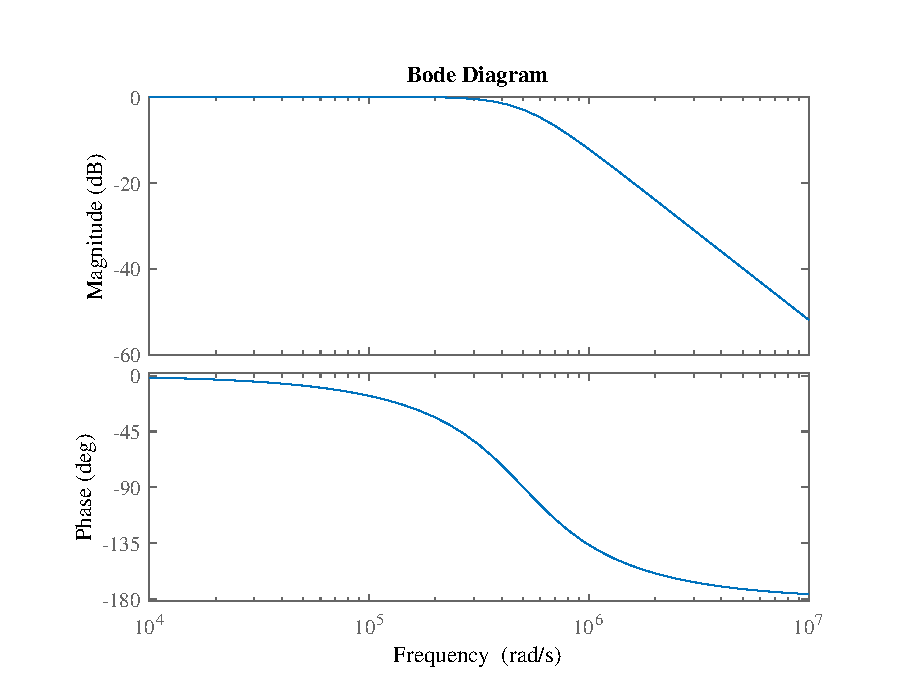
\includegraphics[width=\linewidth]{exp2_matlab_bode}
		\caption{}
	\end{subfigure}
	\begin{subfigure}{0.4\textwidth}
		\centering
		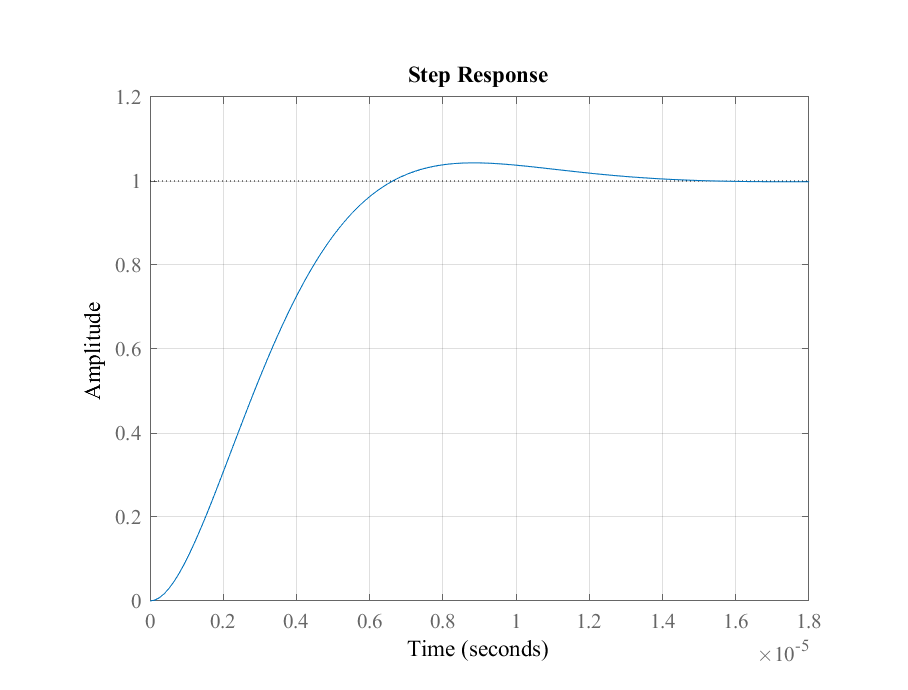
\includegraphics[width=\linewidth]{exp2_matlab_step}
		\caption{}
	\end{subfigure}
	\caption{Using the Control Systems toolbox within MATLAB, the (a) frequency response and (b) step response were captured of the circuit.}
	\label{fig:exp2_matlab}	
\end{figure}
\vspace{-1em}
\begin{figure}[H]
	\centering
	\begin{subfigure}{0.4\textwidth}
		\centering
		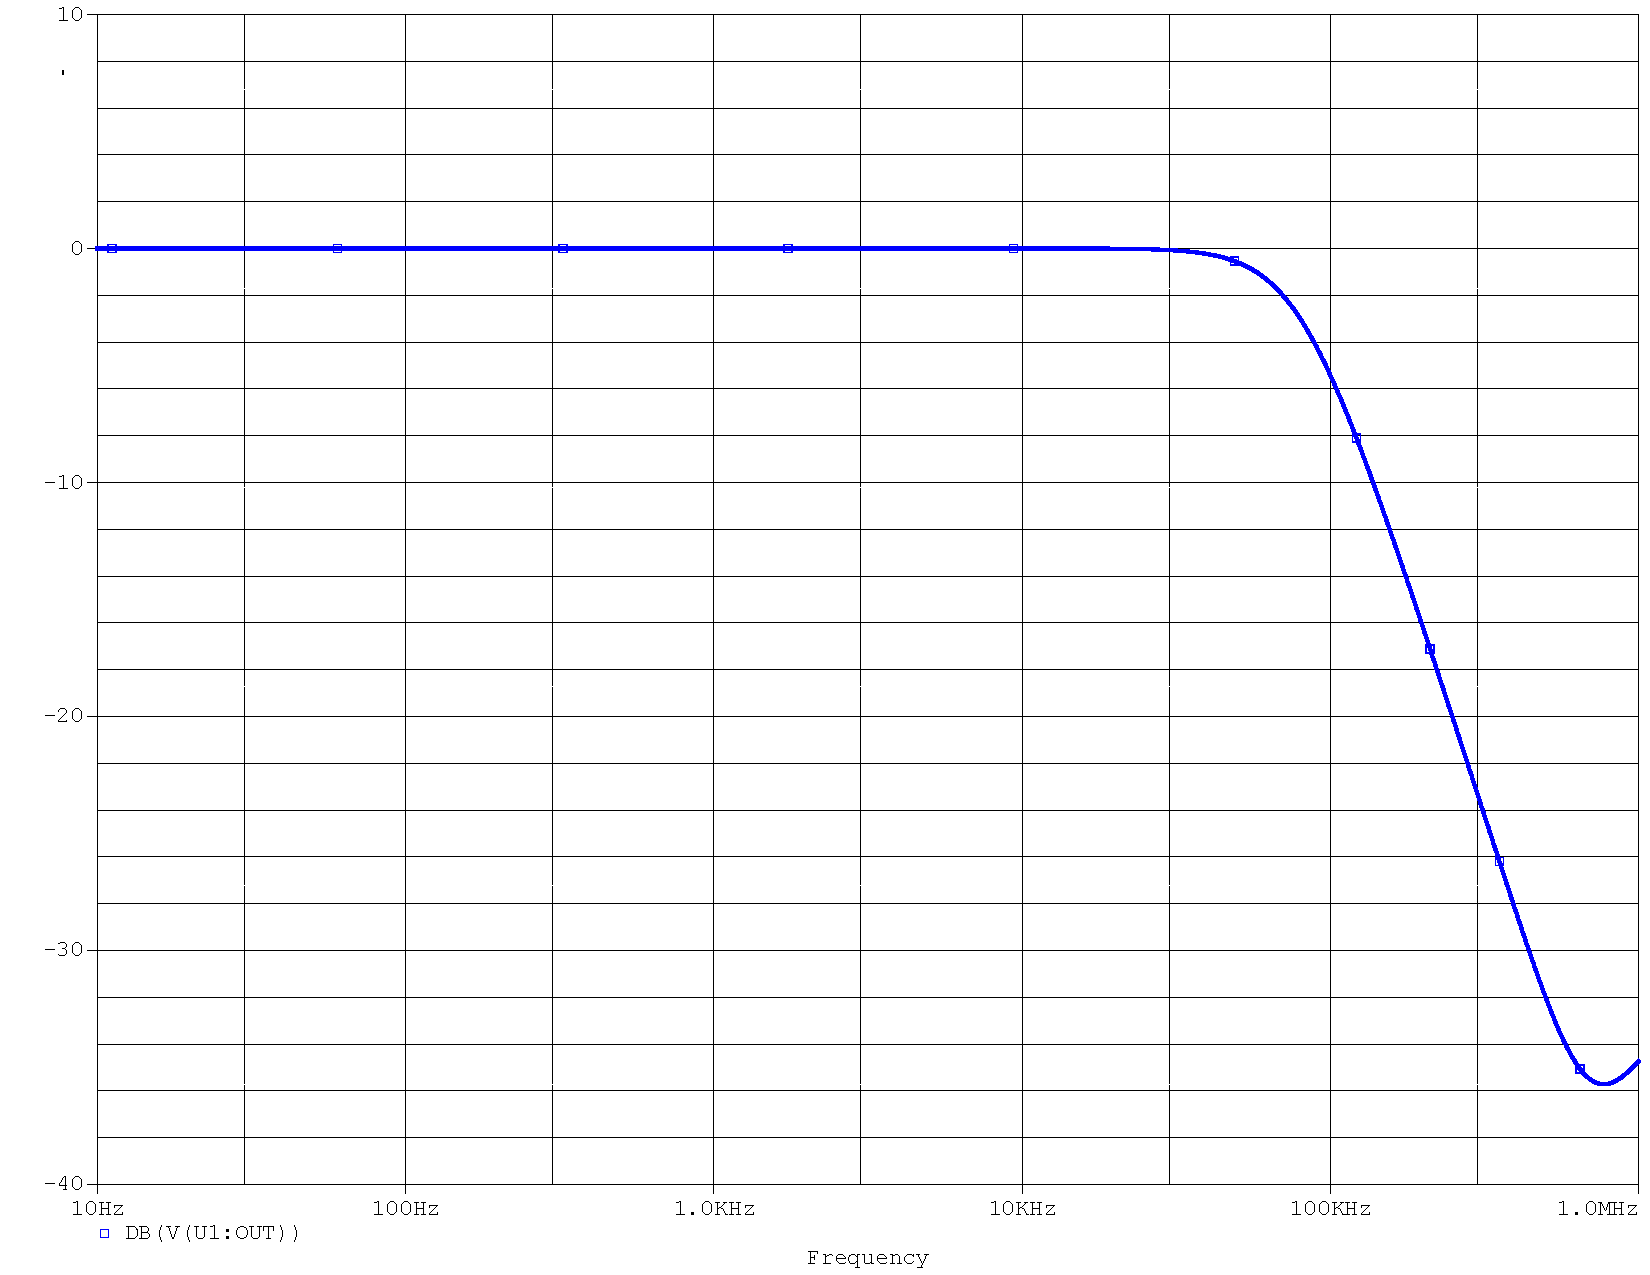
\includegraphics[width=\linewidth]{exp2_orcad_bode}
		\caption{}
	\end{subfigure}
	\begin{subfigure}{0.4\textwidth}
		\centering
		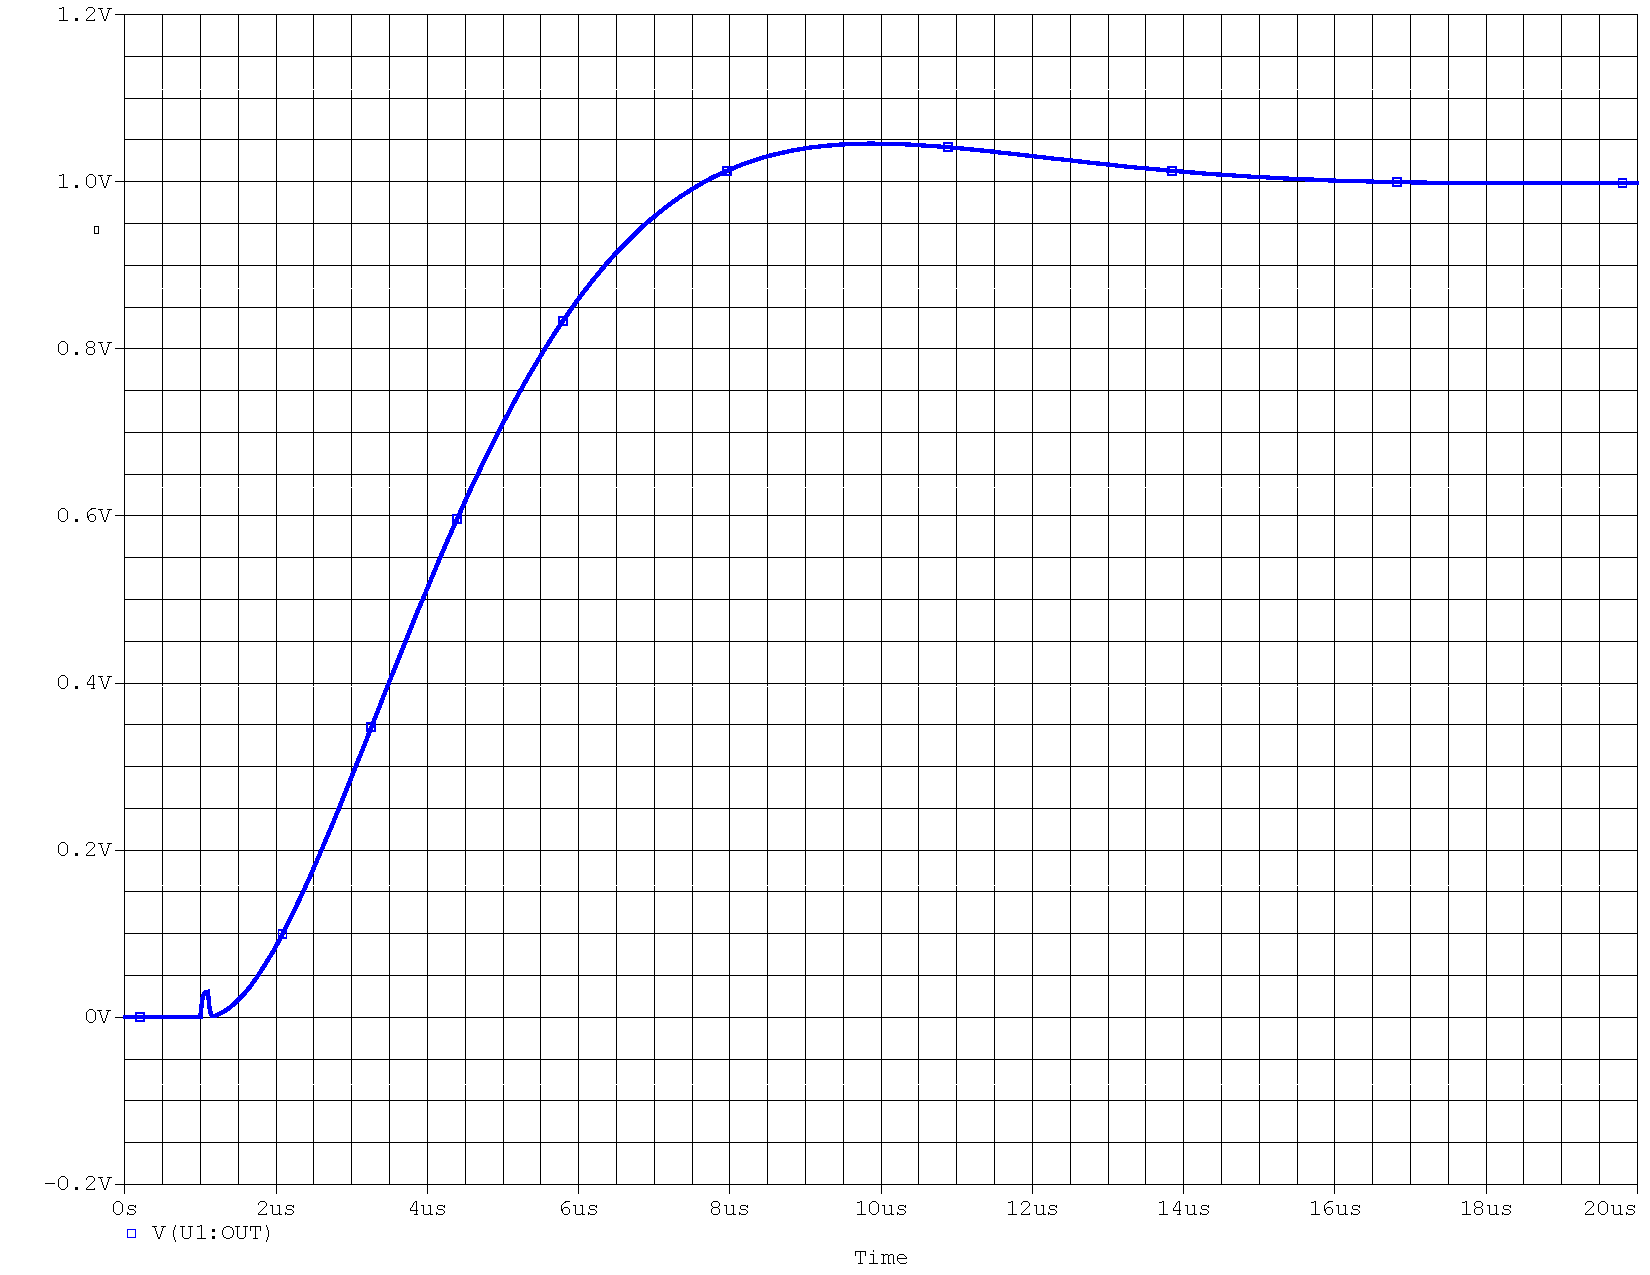
\includegraphics[width=\linewidth]{exp2_orcad_step}
		\caption{}
	\end{subfigure}
	\caption{Using OrCAD PSPICE, a simulation was done for the Butterworth filter, showing the (a) frequency response and (b) step response.}
	\label{fig:exp2_orcad}	
\end{figure}
\subsection{Procedure}
The follow steps were carried out, as instructed by the lab assignment.
\begin{enumerate}
	\item The circuit shown in Figure \ref{fig:exp2ckt} was constructed using the nominal component values determined in the prelab. The OP27 opamp was attached to $\pm$\SI{12}{\V} dc. The component values were measured using the DMM and RLC meter.
	\item The frequency response was experimentally determined. This was done by using a sine wave input of amplitude \SI{8}{\Vpp} and probing the filter's input and output voltages using the oscilloscope. The difference in time between the peaks were determined as well. This data was collected for roughly 20 points and recorded in Excel.
	\item The step response was experimentally determined. We used a square wave of \SI{1}{\Vpp} with a half-volt offset. The step response was sketched and the waveforms were saved on a flash drive.
	\item The circuit was demonstrated to the TA.
\end{enumerate}

\subsection{Results and analysis}
% state all measured values, graphs, tables, and figs.
% state any deviation from theoretical expected values
% use tables and graphs
% * must justify error in results otherwise the experiment failed

\subsubsection{Measured component values}
The components were measured using the DMM and the RLC meter. The component values are shown in Table \ref{table:lab2components} below.
\begin{table}[h]
	\centering
	\caption{Experimental and nominal component values.}
	\label{table:lab2components}
	\begin{threeparttable}
		\begin{tabular}{cccc}
			\toprule
			Component & Nominal & Experimental & \% Error \\
			\midrule
			$R_1$ & \SI{281}{\ohm} & \SI{278.01}{\ohm} & 1.1\% \\
			$R_2$ & \SI{281}{\ohm} & \SI{278.43}{\ohm} & 0.91\% \\
			$C_1$ & \SI{10}{\nano\farad} & \SI{10.45}{\nano\farad} & 4.5\% \\
			$C_2$ & \SI{5}{\nano\farad} & \SI{4.726}{\nano\farad} & 5.5\%\\
			\bottomrule
		\end{tabular}
	\end{threeparttable}
\end{table}
\subsubsection{Frequency response}
Within Excel, the filter's gain and phase differences were recorded. This data was then plotted on a semi-log scale, shown in Figure \ref{fig:exp2bode} below. Notably, the cutoff frequency was determined to be roughly \SI{85}{\kHz}, roughly 6.3\% error from the estimated \SI{80}{\kHz} corner frequency. The error was likely due to the additional internal impedances of the components and non-ideal nature of our setup. Additionally, the higher-than-expected capacitance values may have led to some inaccuracies as the capacitors were rated as ``M'' tolerances, or a 10\% tolerance.

Relative to the simulation, there was some notable differences, including the difference in corner frequency. However, the non-ideal real-world filter exhibited the characteristic Butterworth curve with no overshoot in the gain-frequency response. In the higher frequencies, the plot showed a nearly linear curve, similar to the MATLAB and PSPICE simulation.
\begin{figure}[h]
	\centering
	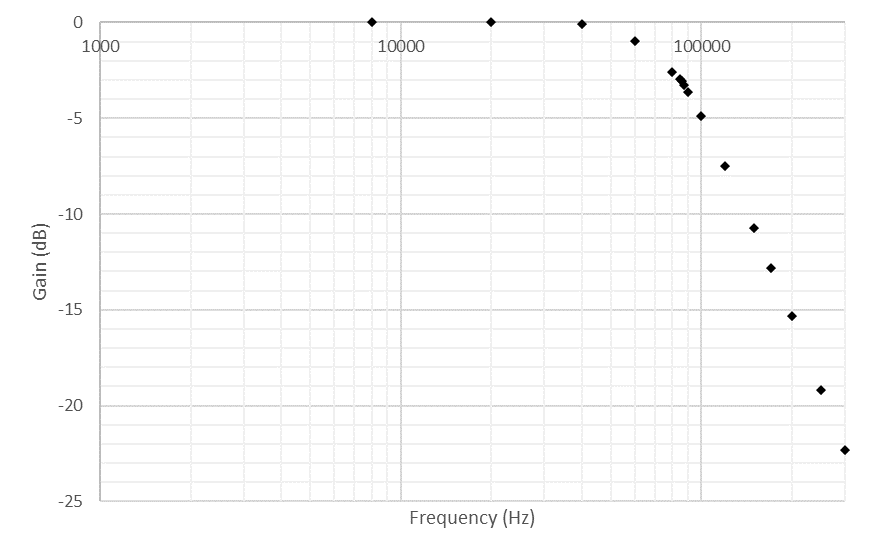
\includegraphics[width=0.5\linewidth]{exp2_freq}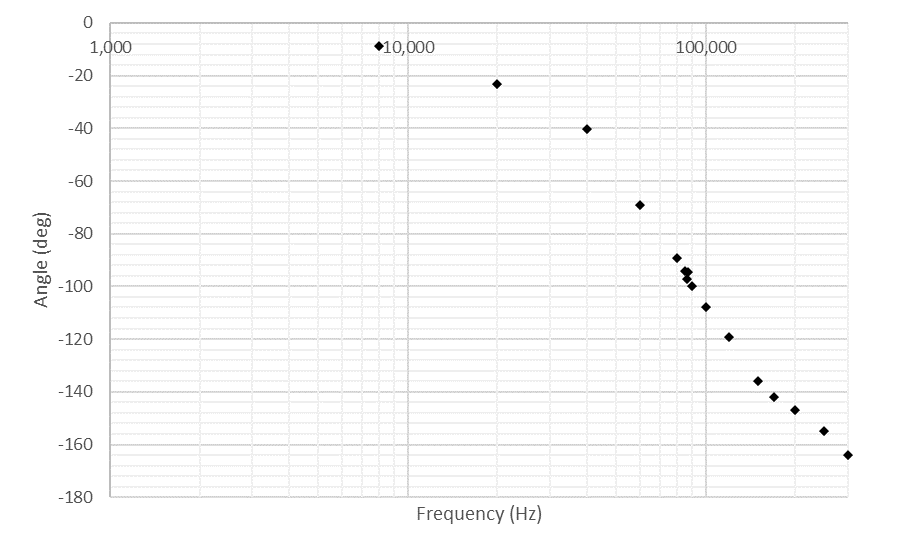
\includegraphics[width=0.5\linewidth]{exp2_angle}
	\caption{Experimental Bode plot of the frequency response of the RLC circuit.}
	\label{fig:exp2bode}
\end{figure}

\subsubsection{Step response}
When applying a square pulse waveform, generally past filters have shown an oscillatory behavior. However, due to the nature of the Butterworth filter, the result is an underdamped response, as shown in Figure \ref{fig:f0004tek}. However, we did notice a half-wave from the start of the impulse to the end of the initial hump, resulting in a $\Delta t = \SI{13.40}{\us}$. However, this was later ruled out as a usable wave. This matched the expected behavior of the MATLAB and PSPICE simulation, as both simulations did not show any oscillatory behavior. The main differences can be attributed to the non-ideal nature of the function generator. In the MATLAB and PSPICE simulation, the step/pulse voltage source is expected to have a zero-duration rise time. However, it is clear from Figure \ref{fig:f0004tek} that the rise-time is several microseconds.
\begin{figure}[h]
	\centering
	\includegraphics[width=0.4\linewidth]{"Lab 6 Pics/F0004TEK"}
	\caption{The underdamped response with no oscillation apparent.}
	\label{fig:f0004tek}
\end{figure}
\subsection{Conclusion}
%  conclusion of the exp
This experiment demonstrated the behavior of the Butterworth filter in a second-order active low-pass application. The frequency response of the filter showed the characteristic Butterworth curve, with a smooth transition between the bandpass region as it reached higher frequencies. The Butterworth filter exhibited no oscillations in the step response, but rather showed an apparent underdamped response. The filter is characterized by the transfer function, which accurately modeled the output voltage to the several types of inputs used in the experiment.


\pagebreak
%%%%%%%%%%%%%%%%%%%%%%%%%%%%%%%%%%%%%%%%%%%%%%%%%%%%%%%%%%%%%
\section{Wide band-pass filter}

\subsection{Purpose}
% purpose of the experiment and its specs and/or design requirements
The purpose of this experiment was to construct a multi-stage filter using the filters created in the past two experiments. This will result in a band-pass with an ideal lower cut-off frequency of \SI{20}{\kHz} and upper-cutoff of \SI{80}{\kHz}. This filter allows us to use characteristics from each and find the resultant transfer function by taking the product of each individual transfer function in the $s$-domain.
\subsection{Theoretical background}
% background and its theory of operation, circuit diagrams, the main equations, results from the prelab
This lab requires the past two filters to be connected serially. Between the two filters will be a buffer, shown in Figure \ref{fig:exp3ckt}. The buffer enables a separation in current between the two filters and gives the first-stage a high-impedance separator, and the low-pass filter is given a low-impedance input.
\begin{figure}[H]
	\centering
	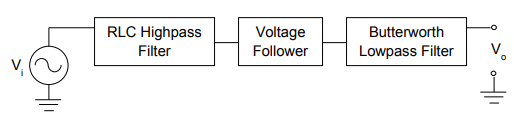
\includegraphics[width=0.5\linewidth]{exp3ckt}
	\caption{A diagram of the circuit setup of the three filter stages.}
	\label{fig:exp3ckt}
\end{figure}
\noindent In the time domain, the stages can be combined using a convolution. However, in the $s$-domain, the transfer function of the band-pass filter can be easily be combined as the product of the two individual filters, \begin{equation}
	H_b(s) = H_h(s) H_\ell(s)
\end{equation}
Using MATLAB, we can use the \texttt{series()} command to combine the earlier-created filters together into a new transfer function, resulting in the transfer function \begin{equation}
H(s) = \frac{ \num{2.527e11} s^2 }
	{s^4 + \num{7.611e05} s^3 + \num{3.042e11}s^2 + \num{2.393e16} s + \num{3.991e21}}
\end{equation}
We can again use MATLAB and plot this. This results in a filter acting as a combination of the earlier filters and acts as a bandpass filter, shown in Figure \ref{fig:exp3_matlab} below.
\begin{figure}[h]
	\centering
	\begin{subfigure}{0.45\textwidth}
		\centering
		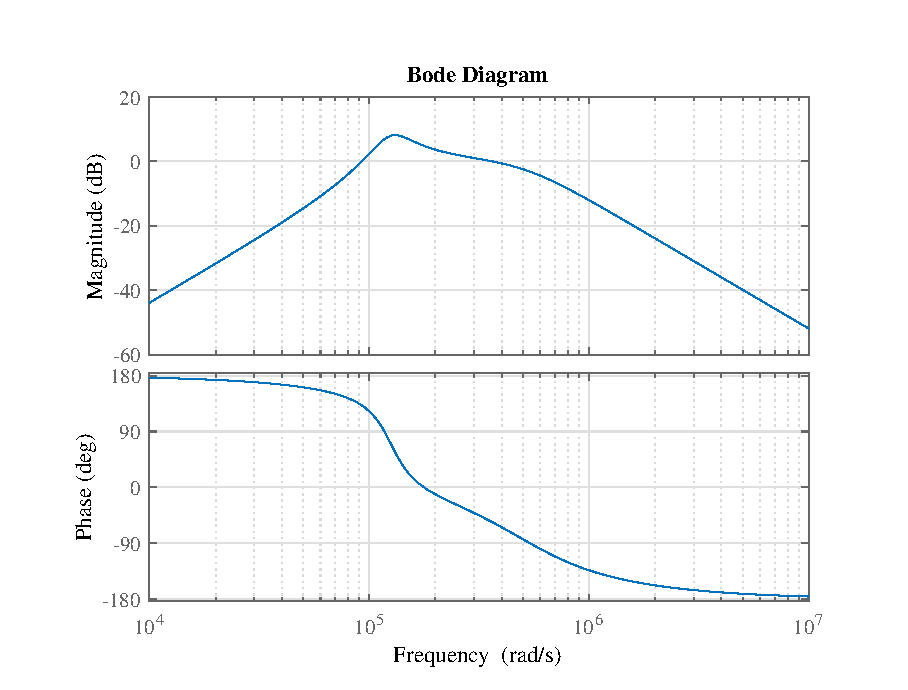
\includegraphics[width=\linewidth]{exp3_matlab_bode}
		\caption{}
	\end{subfigure}
	\begin{subfigure}{0.45\textwidth}
		\centering
		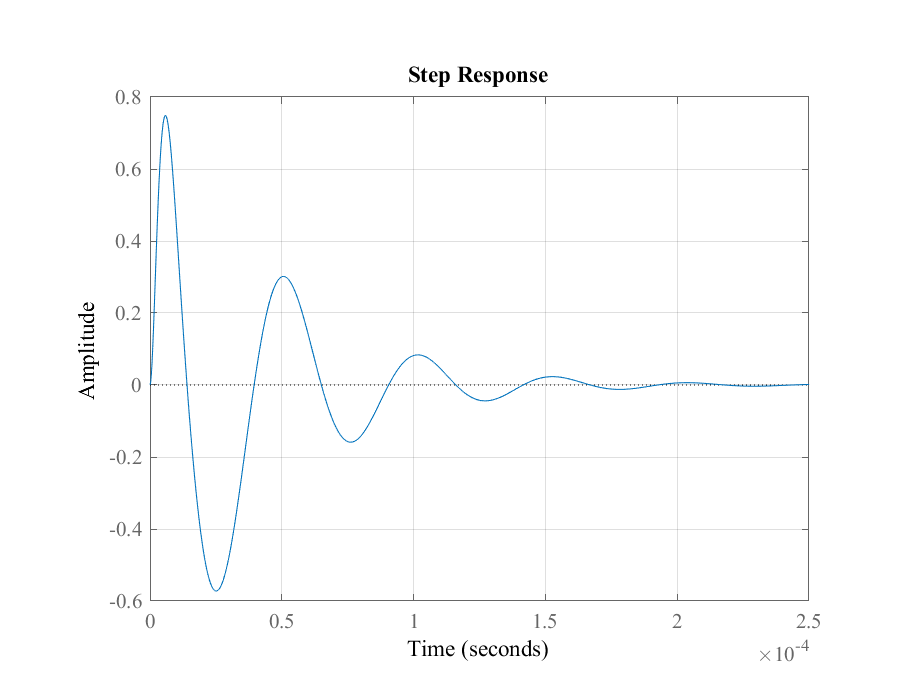
\includegraphics[width=\linewidth]{exp3_matlab_step}
		\caption{}
	\end{subfigure}
	\caption{Using the Control Systems toolbox within MATLAB, the (a) frequency response and (b) step response were captured of the circuit.}
	\label{fig:exp3_matlab}	
\end{figure}
\subsection{Procedure}
The follow steps were carried out, as instructed by the lab assignment.
\begin{enumerate}
	\item The circuit was attached per the diagram in Figure \ref{fig:exp3ckt}. The earlier filters were attached with an OP27 opamp acting as a buffer (with unity gain) between each circuit. The opamp was attached to $\pm$\SI{12}{\Vpp} as the power supply. 
	\item Using a \SI{4}{\Vpp} sine wave, the amplitude frequency response was determined and recorded in Excel. Unlike the past experiments, the phase response was not recorded. In this experiment, we included the \SI{50}{\ohm} resistor in the first filter, as done in Experiment 1. The frequencies ranged between \SI{2}{\kHz} to \SI{300}{\kHz}.
	\item Next, the step response of the circuit was experimentally determined using a \SI{1}{\Vpp} square wave with a dc offset of \SI{0.5}{\V}. The \SI{50}{\ohm} resistor was removed again for this experiment. The oscillatory behavior was noted and the oscilloscope screen was saved onto a Flash drive.
	\item This was demonstrated to the TA.
\end{enumerate}

\subsection{Results and analysis}
% state all measured values, graphs, tables, and figs.
% state any deviation from theoretical expected values
% use tables and graphs
% * must justify error in results otherwise the experiment failed

\subsubsection{Frequency response}
Roughly 20 data points were collected in Excel and plotted on a semi-log scale. The maximum gain was roughly around \SI{20}{\kHz} with \SI{5.85}{\dB} gain. As the frequency increased, the gain was reduced. At \SI{80}{\dB}, the gain was approximately \SI{-0.18}{\dB}. Around \SI{86}{\kHz}, the gain was attenuated to \SI{-2.92}{\dB}. The full measured response is shown in Figure \ref{fig:exp3freq}.
\begin{figure}[h]
	\centering
	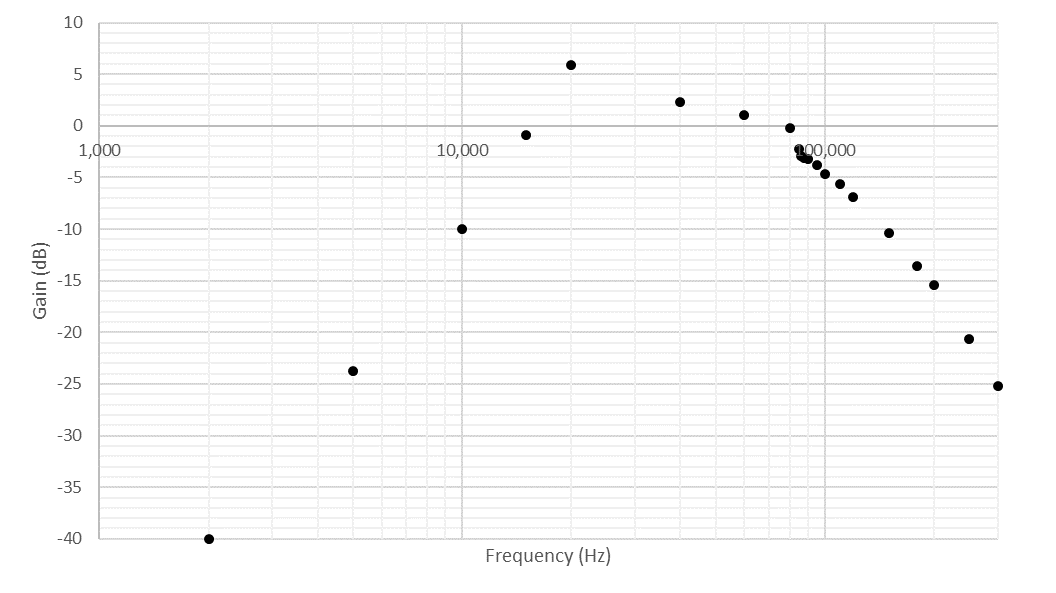
\includegraphics[width=0.7\linewidth]{exp3freq}
	\caption{Frequency response of the three-stage bandpass filter.}
	\label{fig:exp3freq}
\end{figure}
\pagebreak
\subsubsection{Step response}
Using the square pulse function on the generator at \SI{1}{\Vpp} with a half-volt offset, oscillatory behavior was observed on the filter's output, shown in Figure \ref{fig:f0006tek} below. Between the first two peaks, the time period and frequency is measured \begin{align*}
	\Delta T & = \SI{43.60}{\us} \\
	f & = \SI{22.94}{\kHz}
\end{align*}
This frequency is seemingly much closer to the natural frequency of the high-pass filter of \SI{21.2}{\kHz}. This seems to be as the oscillations of the step response from the first high-pass filter were much more evident than the oscillations of the low-pass Butterworth filter. 
\begin{figure}[h]
	\centering
	\includegraphics[width=0.4\linewidth]{"Lab 6 Pics/F0006TEK"}
	\caption{The step response of the combination filter.}
	\label{fig:f0006tek}
\end{figure}

\subsection{Conclusion}
%  conclusion of the exp
Filters can be attached serially and the transfer function of the cascaded filters becomes a product of the transfer functions of each individual filter in the $s$-domain. Combining filters allows us to take parts of each individual filter and juxtapose the filters to create one filter with desirable characteristics of each. In this experiment, we combined a low-pass and a high-pass filter, enabling a new bandpass filter with a nearly-linear ramp up to a slight damping $\zeta$ constant and a smooth Butterworth transition at higher frequencies. The step response showed a response with a combination of both individual filter's step responses, demonstrating that the high-pass filter was much more visible and retained in the serially connected filter, than the underdamped step response of the Butterworth filter.


\pagebreak
\section*{Appendix}
\subsubsection{MATLAB code used to acquire and simulate the transfer functions.}
\begin{lstlisting}[language=matlab]
L = 1e-3;    % henry
C = 63.3e-9; % farad
R = 50.26;   % ohm

N = [1, 0,     0      ]; % numerator coefficients
D = [1, (R/L), 1/(L*C)]; % denomenator coefficients

Hsys1 = tf(N, D);
step(Hsys1);
grid;
figure;
bode(Hsys1);
grid;

%%%%%%%%%%%%%%%%%%%%%%%
% Exp. 2/3   %        %
C1 = 10e-9;  % farad  %
C2 =  5e-9;  % farad  %
R  = 281.35; % ohm    %
%%%%%%%%%%%%%%%%%%%%%%%


N = [0,            0, 1 / (R.^2 * C1 * C2)]; % numerator coefficients
D = [1, 2 / (R * C1), 1 / (R.^2 * C1 * C2)]; % denomenator coefficients

Hsys2 = tf(N, D);

step(Hsys2);
grid on;


Hbandpass = series(Hsys1, Hsys2);
bode(Hbandpass);
grid on;
figure;
step(Hbandpass);
grid on;
\end{lstlisting}
\end{document}